% D. Plummer and A. Kovaľ, Strongly regular graphs on 442 points from line pieces in two conference two-graphs.
% Build: pdflatex main && pdflatex main.  Programs and data: https://github.com/dylan-plummer/srg442-line-pieces
\documentclass[11pt]{amsart}
\usepackage[T1]{fontenc}
\usepackage{lmodern}
\usepackage[margin=25mm]{geometry}
\usepackage{amssymb,amsmath,amsthm,booktabs,graphicx,microtype}
\usepackage{xcolor}
\usepackage{placeins}
\usepackage{tikz}
\usetikzlibrary{positioning,calc,arrows.meta,fit,backgrounds}
\usepackage[hidelinks]{hyperref}
\graphicspath{{figures/}}
\emergencystretch=2em

\newtheorem{theorem}{Theorem}[section]
\newtheorem{lemma}[theorem]{Lemma}
\newtheorem{proposition}[theorem]{Proposition}
\newtheorem{corollary}[theorem]{Corollary}
\newtheorem{conjecture}[theorem]{Conjecture}
\theoremstyle{definition}
\newtheorem{definition}[theorem]{Definition}
\theoremstyle{remark}
\newtheorem{remark}[theorem]{Remark}
\newtheorem{question}[theorem]{Question}

\newcommand{\F}{\mathbb{F}}
\newcommand{\Z}{\mathbb{Z}}
\newcommand{\srg}{\mathrm{srg}}
\newcommand{\Aut}{\mathrm{Aut}}
\newcommand{\Pal}{\mathrm{Paley}}
\newcommand{\one}{\mathbf 1}
\newcommand{\code}[1]{\texttt{#1}}
\newcommand{\OM}{\Omega_{\mathrm M}}   % Mathon's two-graph
\newcommand{\OP}{\Omega_{\mathrm P}}   % the variant with Paley(49) fibres (A.K.'s proposal, 16 Nov 2026)
\newcommand{\todo}[1]{{\color{red}[TODO: #1]}}

\title[Strongly regular graphs on 442 points]{Strongly regular graphs on $442$ points from line pieces
in two conference two-graphs}
\author{Dylan Plummer}
\author{Anton Kova\v{l}}
\date{19 November 2026}



\begin{document}
\begin{abstract}
We construct $2356$ pairwise non-isomorphic strongly regular graphs with parameters $(442,231,120,121)$; their
complements have parameters $(442,210,99,100)$. They come from two regular two-graphs on $442$ points, Mathon's
conference two-graph $\OM$ and a variant $\OP$ whose fibres are copies of $\Pal(49)$: $2\cdot575$ of them are regular
members of degree $231$, and $2\cdot603$ are complements of regular members of degree $210$. Both are instances of one
template for conference two-graphs on $pq^2+1$ points, in which all points but one are partitioned into $p$ fibres,
each a copy of the affine plane $\F_q^2$. Each of our graphs is obtained by switching with respect to a set that meets
every fibre in a union of parallel lines. The fibres that such a set meets non-trivially occur in pairs, and this lets
us enumerate all such graphs. For each two-graph and degree the $5145$ such switching sets fall into $15$ frames, and each
frame contains exactly one that is invariant under the subgroup of order $3$ of automorphisms fixing every fibre.

A regular graph in a template two-graph requires $p=s^2$, so $q=s^2-2$, and $q=7$ is the first case. We show that the
structure found at $q=7$ does not extend to larger $q$ for standard line pieces: it needs a character sum that takes
exactly two values differing by $s\pm1$, and standard line pieces provide one only for $s=3$. For arbitrary line pieces
this rests on a conjecture on two-valued character sums over $\F_q$, $q$ prime, except at $q=23$, where we prove it. At $q=23$ ($13226$ points) no
two-graph of the template has a regular member whose switching set meets every fibre in a union of parallel lines, and
Mathon's two-graph on $13226$ points (base $\Pal(25)$, circulant skew Latin square) has no regular member invariant
under its scalar automorphism.
\end{abstract}
\maketitle

\section{Introduction}\label{sec:intro}
A strongly regular graph $\srg(v,k,\lambda,\mu)$ is a $k$-regular graph on $v$ vertices, neither complete nor edgeless, in
which any two adjacent vertices have exactly $\lambda$ common neighbours and any two distinct non-adjacent vertices exactly
$\mu$; see~\cite{BvM2022}. The parameter sets $(442,231,120,121)$ and $(442,210,99,100)$ were open in Brouwer's
table~\cite{BrouwerTable} until~\cite{Plummer442}. No such graph is a Cayley graph~\cite[Appendix~B]{NelsonSwartz2025}. Since
$v=2(2k-\lambda-\mu)$, a graph with these parameters is a regular graph in a regular two-graph on $442$ points, and its
Seidel matrix is a symmetric conference matrix of order $442$~\cite[\S\S10.3--10.4]{BH2012}. Since $442=9\cdot7^2+1$, Mathon's
construction~\cite{Mathon1978} gives one; \cite{Plummer442} found $14$ regular graphs in its switching class whose switching sets
meet every fibre in a union of parallel lines. Here we find all such graphs, in this and in a second two-graph, and
show that the line-piece construction does not continue to larger orders: for standard line pieces in general, for all
line pieces at $q=23$, and for arbitrary line pieces beyond $q=23$ conditionally on Conjecture~\ref{conj:twoval}. We do not know whether these two-graphs have regular
members outside the line-piece model.

In this paper we place Mathon's two-graph in a template of conference two-graphs on $pq^2+1$ points
(Definition~\ref{def:template}), which also contains a second two-graph $\OP$ with $\Pal(49)$ fibres and at least $21$ further
two-graphs on $442$ points. Our results are:
\begin{enumerate}
\item a complete census of the \emph{line-piece} regular members of $\OM$ and $\OP$: $2356$ pairwise non-isomorphic strongly
regular graphs (Theorem~\ref{thm:census}); the $5145$ line-piece members of each two-graph and degree are organised by
decoupled pairs of fibres into $15$ frames, each with exactly one centred member (Section~\ref{sec:census});
\item the line pieces are sporadic for $q=s^2-2$: a line piece whose intercept set is a translate of a union of
$\{0\}$, $Q$, $N$ can occur in a line-piece regular member only if a character sum is two-valued with gap $s\pm1$, which happens
only for $s=3$, i.e.\ $q=7$ (Theorem~\ref{thm:sporadic}); for arbitrary intercept sets this rests on
Conjecture~\ref{conj:twoval};
\item at $q=23$ ($13226$ points) no two-graph of the template has a line-piece regular member
(Proposition~\ref{prop:q23all}), and Mathon's two-graph on $\Pal(25)$ with the circulant square has no regular member
invariant under its scalar automorphism (Proposition~\ref{prop:q23h}).
\end{enumerate}

Figure~\ref{fig:flow} gives the structure of the paper: from the template (Section~\ref{sec:template}) through
line-piece switching and decoupling to the census (Section~\ref{sec:census}), and the sporadicity of the line-piece
members in Mathon's family (Section~\ref{sec:sporadic}). Section~\ref{sec:verification} lists the programs behind every
computational statement.

\begin{figure}[t]
\centering
\resizebox{0.95\textwidth}{!}{% Flowchart: inputs -> template -> regular two-graphs on 442 points -> line-piece members -> census -> the 2356 graphs.
% \input this inside a figure; needs \usetikzlibrary{positioning,calc,arrows.meta,fit,backgrounds} and \F, \srg, \Aut.
% Color code as in Figure 2: blue = line(s) in a net direction, orange = outside the net, gray = whole fiber.
% The small drawings use the example member of Figure 2 (its pair 0 -> 3 and its frame).
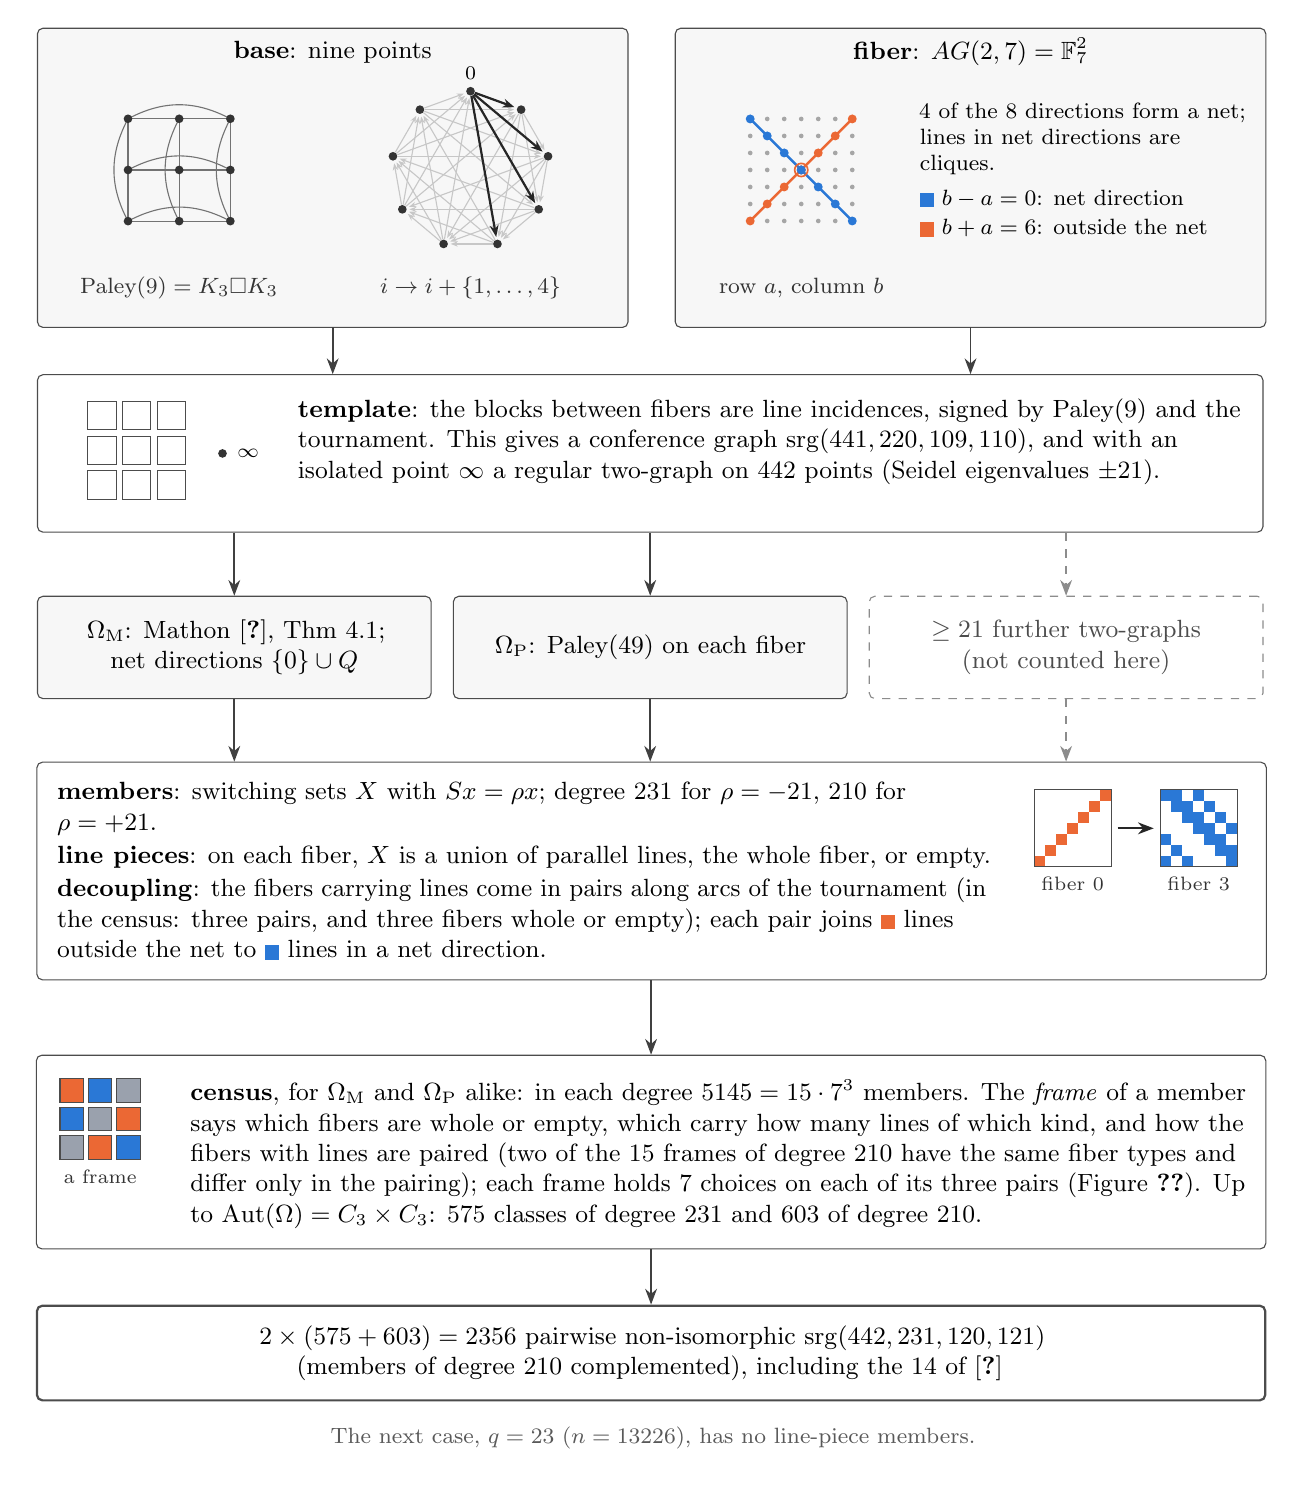
\begin{tikzpicture}[x=1mm, y=1mm, font=\small,
  box/.style={draw=black!70, rounded corners=2pt},
  inbox/.style={box, fill=black!3},
  fitbox/.style={box, inner sep=2.5mm},
  txt/.style={inner sep=0pt, align=flush left},
  ctxt/.style={inner sep=0pt, align=flush center},
  ibox/.style={box, fill=black!3, inner sep=2.5mm, align=flush center, text width=45mm, minimum height=13mm},
  fbox/.style={ibox, fill=none, draw=black!45, dashed, text=black!70},
  arr/.style={-{Stealth[length=2mm]}, semithick, draw=black!75},
  dot/.style={circle, fill=black!80, inner sep=0pt, minimum size=1.1mm},
  lab/.style={ctxt, font=\footnotesize, text=black!80},
  note/.style={font=\footnotesize, text=black!65}]
\definecolor{cnet}{HTML}{2A78D6}\definecolor{cnon}{HTML}{EB6834}\definecolor{cwhole}{HTML}{9AA1AD}
\newcommand{\sw}[1]{\textcolor{#1}{\rule[-0.2ex]{1.8mm}{1.8mm}}}

% =========================================================================== inputs
\draw[inbox] (0,3) rectangle (75,-35);
\node[ctxt] at (37.5,0) {\textbf{base}: nine points};
\begin{scope}[shift={(18,-15)}]                                  % Paley(9) = K3 x K3; point i at row i div 3, column i mod 3
  \foreach \r in {0,1,2} \foreach \c in {0,1,2} \coordinate (p\r\c) at (6.5*\c-6.5, -6.5*\r+6.5);
  \foreach \r in {0,1,2} {\draw[black!55] (p\r0)--(p\r1)--(p\r2); \draw[black!55] (p\r0) to[bend left=28] (p\r2);}
  \foreach \c in {0,1,2} {\draw[black!55] (p0\c)--(p1\c)--(p2\c); \draw[black!55] (p0\c) to[bend right=28] (p2\c);}
  \foreach \r in {0,1,2} \foreach \c in {0,1,2} \node[dot] at (p\r\c) {};
  \node[lab] at (0,-15) {Paley$(9)=K_3\square K_3$};
\end{scope}
\begin{scope}[shift={(55,-15)}]                                  % the tournament i -> i+{1,...,4}; the arcs out of 0 dark
  \foreach \i in {0,...,8} \coordinate (t\i) at ({90-40*\i}:10);
  \foreach \i in {1,...,8} \foreach \d in {1,...,4} {
    \pgfmathtruncatemacro\j{mod(\i+\d,9)}
    \draw[black!22, -{Stealth[length=0.9mm]}, shorten >=0.9mm, shorten <=0.6mm] (t\i)--(t\j);}
  \foreach \d in {1,...,4} \draw[black!85, thick, -{Stealth[length=1.5mm]}, shorten >=0.9mm, shorten <=0.6mm] (t0)--(t\d);
  \foreach \i in {0,...,8} \node[dot] at (t\i) {};
  \node[font=\scriptsize] at (0,12.3) {$0$};
  \node[lab] at (0,-15) {$i\to i+\{1,\dots,4\}$};
\end{scope}

\draw[inbox] (81,3) rectangle (156,-35);
\node[ctxt] at (118.5,0) {\textbf{fiber}: $AG(2,7)=\F_7^2$};
\begin{scope}[shift={(97,-15)}]                                  % 7 x 7 points, row a, column b
  \begin{scope}[scale=1.35]
  \foreach \a in {0,...,6} \foreach \b in {0,...,6} \fill[black!35] (1.6*\b-4.8, -1.6*\a+4.8) circle (0.22);
  \draw[cnet, line width=0.9pt] (-4.8,4.8) -- (4.8,-4.8);                       % b - a = 0
  \draw[cnon, line width=0.9pt] (4.8,4.8) -- (-4.8,-4.8);                       % b + a = 6
  \foreach \a in {0,...,6} {\fill[cnet] (1.6*\a-4.8, -1.6*\a+4.8) circle (0.42); \fill[cnon] (4.8-1.6*\a, -1.6*\a+4.8) circle (0.42);}
  \fill[cnet] (0,0) circle (0.42); \draw[cnon, line width=0.6pt] (0,0) circle (0.62);
  \end{scope}
  \node[lab] at (0,-15) {row $a$, column $b$};
\end{scope}
\node[txt, text width=41mm, font=\footnotesize, anchor=west] at (112,-15)
  {$4$ of the $8$ directions form a net; lines in net directions are cliques.\\[3pt]
   \sw{cnet}\ $b-a=0$: net direction\\[1pt]
   \sw{cnon}\ $b+a=6$: outside the net};

% =========================================================================== template
\node[txt, text width=120mm, anchor=north west] (tT) at (33,-44)
  {\textbf{template}: the blocks between fibers are line incidences, signed by Paley$(9)$ and the tournament.
   This gives a conference graph $\srg(441,220,109,110)$, and with an isolated point $\infty$ a regular two-graph
   on $442$ points (Seidel eigenvalues $\pm21$).};
\begin{scope}[shift={(13,-51)}]                                   % nine fibers on the base, and oo
  \foreach \i in {0,...,8} {\pgfmathtruncatemacro\r{\i/3}\pgfmathtruncatemacro\c{mod(\i,3)}
    \draw[black!70, fill=white] (4.4*\c-6.6, -4.4*\r+6.6) rectangle ++(3.6,-3.6);}
  \node[dot] (oo) at (10.5,0) {}; \node[font=\scriptsize, right] at (oo.east) {$\infty$};
  \coordinate (ti1) at (-10.5,7.5); \coordinate (ti2) at (14,-7.5);
\end{scope}
\begin{scope}[on background layer]\node[fitbox, fill=white, fit=(tT)(ti1)(ti2)] (T) {};\end{scope}
\draw[arr] (37.5,-35) -- (37.5,0 |- T.north);
\draw[arr] (118.5,-35) -- (118.5,0 |- T.north);

% =========================================================================== instances
\node[ibox, below=8mm of T.south west, anchor=north west] (OM)
  {$\Omega_{\mathrm M}$: Mathon \cite{Mathon1978}, Thm~4.1;\\ net directions $\{0\}\cup Q$};
\node[ibox, below=8mm of T.south, anchor=north] (OK)
  {$\Omega_{\mathrm P}$: Paley$(49)$ on each fiber};
\node[fbox, below=8mm of T.south east, anchor=north east] (OF)
  {$\ge21$ further two-graphs\\ (not counted here)};
\foreach \n in {OM, OK} \draw[arr] (T.south -| \n) -- (\n.north);
\draw[arr, dashed, draw=black!45] (T.south -| OF) -- (OF.north);

% =========================================================================== members
\node[txt, text width=118mm, anchor=north west] (mT) at ($(OM.south west)+(2.5,-10.5)$)
  {\textbf{members}: switching sets $X$ with $Sx=\rho x$; degree $231$ for $\rho=-21$, $210$ for $\rho=+21$.\\[1pt]
   \textbf{line pieces}: on each fiber, $X$ is a union of parallel lines, the whole fiber, or empty.\\[1pt]
   \textbf{decoupling}: the fibers carrying lines come in pairs along arcs of the tournament (in the census:
   three pairs, and three fibers whole or empty); each pair joins \sw{cnon}\ lines outside the net to \sw{cnet}\ lines in a net direction.};
\begin{scope}[shift={($(mT.north east)+(6,-1)$)}]                  % the pair 0 -> 3 of Figure 2
  \foreach \a in {0,...,6} \foreach \b in {0,...,6} {
    \pgfmathtruncatemacro\u{mod(\a+\b,7)==6}\pgfmathtruncatemacro\v{or(or(mod(\b-\a+7,7)==0, mod(\b-\a+7,7)==1), mod(\b-\a+7,7)==3)}
    \ifnum\u=1 \fill[cnon] (1.4*\b, -1.4*\a) rectangle ++(1.4,-1.4); \fi
    \ifnum\v=1 \fill[cnet] (1.4*\b+16, -1.4*\a) rectangle ++(1.4,-1.4); \fi}
  \draw[black!70] (0,0) rectangle (9.8,-9.8); \draw[black!70] (16,0) rectangle (25.8,-9.8);
  \draw[arr, thick, draw=black!85] (10.6,-4.9) -- (15.2,-4.9);
  \node[lab, font=\scriptsize] at (4.9,-12) {fiber $0$}; \node[lab, font=\scriptsize] at (20.9,-12) {fiber $3$};
  \coordinate (mi) at (27,-13.5);
\end{scope}
\begin{scope}[on background layer]\node[fitbox, fill=white, fit=(mT)(mi)] (P) {};\end{scope}
\foreach \n in {OM, OK} \draw[arr] (\n.south) -- (\n.south |- P.north);
\draw[arr, dashed, draw=black!45] (OF.south) -- (OF.south |- P.north);

% =========================================================================== census
\begin{scope}[shift={($(P.south west)+(3,-12.5)$)}]              % the frame of the member of Figure 2
  \foreach \i/\k in {0/cnon,1/cnet,2/cwhole,3/cnet,4/cwhole,5/cnon,6/cwhole,7/cnon,8/cnet} {
    \pgfmathtruncatemacro\r{\i/3}\pgfmathtruncatemacro\c{mod(\i,3)}
    \draw[black!70, fill=\k] (3.6*\c, -3.6*\r) rectangle ++(3,-3);}
  \node[lab, font=\scriptsize] at (5.1,-12.4) {a frame};
  \coordinate (ci1) at (-0.5,0.5); \coordinate (ci2) at (10.6,-13.4);
\end{scope}
\node[txt, text width=134mm, anchor=north west] (cT) at ($(ci1)+(17,-0.5)$)
  {\textbf{census}, for $\Omega_{\mathrm M}$ and $\Omega_{\mathrm P}$ alike: in each degree $5145=15\cdot7^3$ members.
   The \emph{frame} of a member says which fibers are whole or empty, which carry how many lines of which kind, and how
   the fibers with lines are paired (two of the $15$ frames of degree $210$ have the same fiber types and differ only in the
   pairing); each frame holds $7$ choices on each of its three pairs (Figure~\ref{fig:member}).
   Up to $\Aut(\Omega)=C_3\times C_3$: $575$ classes of degree $231$ and $603$ of degree $210$.};
\begin{scope}[on background layer]\node[fitbox, fill=white, fit=(cT)(ci1)(ci2)] (C) {};\end{scope}
\draw[arr] (P.south -| C.north) -- (C.north);

% =========================================================================== result
\node[box, line width=0.8pt, inner sep=2.5mm, text width=151mm, align=flush center, below=7mm of C] (all)
  {$2\times(575+603)=2356$ pairwise non-isomorphic $\srg(442,231,120,121)$\\
   (members of degree $210$ complemented), including the $14$ of \cite{Plummer442}};
\draw[arr] (C) -- (all);
\node[note, text width=156mm, below=2mm of all, align=flush center]
  {
   The next case, $q=23$ ($n=13226$), has no line-piece members.};
\end{tikzpicture}
}
\caption{From the template to the $2356$ graphs.
The drawings use the colour code and the example member of Figure~\ref{fig:member}.
Other choices of the template data give at least $23$ pairwise inequivalent two-graphs in all (dashed box); only $\OM$
\cite{Mathon1978} and $\OP$ are counted here. We do not classify members outside the line-piece model.}
\label{fig:flow}
\end{figure}

\section{The template}\label{sec:template}

Let $q\equiv3\pmod4$ be a prime and $p=q+2$, so $n=pq^2+1$. Let $Q$, $N$ be the non-zero squares and non-squares of $\F_q$
and $V=\F_q^2$; its $q+1$ one-dimensional subspaces are the \emph{lines}, and a non-zero linear form $f$ is determined by
$\ker f$ up to a factor in $\F_q^\times$. Seidel matrices are taken for a graph on $n-1$ vertices together with an isolated
point $\infty$. For $x\in\{\pm1\}^n$ with $x_\infty=1$, the graph switched by $x$ is regular of degree $k$ if and only if
$Sx=\rho x$ with $\rho=n-1-2k$, and it is then strongly regular~\cite{Seidel1976,Taylor1977},~\cite[\S10.3]{BH2012}.

\begin{definition}[template]\label{def:template}
Let $\Delta$ be a conference graph on a set $B$ of $p$ vertices, $\varepsilon_{ab}=+1$ on edges and $-1$ on non-edges.
\emph{Template data} consist of
\begin{enumerate}
\item[(T1)] for each $i\in B$ a set $\mathcal L_i$ of $(q+1)/2$ lines; the fibre $\Phi_i$ is the Cayley graph on
$(V,+)$ with connection set $\bigcup_{L\in\mathcal L_i}L\setminus\{0\}$, a strongly regular graph of Latin square
type~\cite{CalderbankKantor1986};
\item[(T2)] a regular tournament on $B$;
\item[(T3)] for each arc $a\to b$ non-zero linear forms $f^+_{ab}$ (tail) and $f^-_{ab}$ (head), such that at every $i$
the kernels of the out-arc forms are exactly the lines not in $\mathcal L_i$, each once, and the kernels of the in-arc
forms are exactly the lines in $\mathcal L_i$, each once;
\item[(T4)] for each arc a set $T_{ab}=\alpha Q+\beta$ if $\varepsilon_{ab}=+1$ and $\alpha(\{0\}\cup N)+\beta$ if
$\varepsilon_{ab}=-1$ ($\alpha\in\F_q^\times$, $\beta\in\F_q$).
\end{enumerate}
The graph has vertex set $B\times V$, fibre $\Phi_i$ on $\{i\}\times V$, and $(a,u)\sim(b,v)$ for an arc $a\to b$ iff
$f^+_{ab}(u)-f^-_{ab}(v)\in T_{ab}$.
\end{definition}

\begin{lemma}\label{lem:blocks}
For a line $D$ let $F^D$ be the space of functions $\varphi\circ\theta$ on $V$ with $\ker\theta=D$ and
$\sum_s\varphi(s)=0$; the functions on $V$ split as $\langle\one\rangle\oplus\bigoplus_DF^D$ (dimensions
$1+(q+1)(q-1)=q^2$). The blocks of $S$ are $S_{\infty i}=\one^\top$, $S_{ii}=J-I-2A(\Phi_i)$ and, for an arc $a\to b$,
$S_{ab}=J-2E_{ab}$ with $E_{ab}(u,v)=[f^+_{ab}(u)-f^-_{ab}(v)\in T_{ab}]$, and $S_{ba}=S_{ab}^\top$. For all template data:
\begin{enumerate}
\item[(F1)] $S_{ii}\one=0$, and $S_{ii}$ acts on $F^D$ by $-q$ if $D\in\mathcal L_i$ and by $+q$ if $D\notin\mathcal L_i$.
\item[(F2)] $S_{ab}\one=\varepsilon_{ab}q\one$ for $a\ne b$.
\item[(F3)] Let $a\to b$ be an arc and $T=T_{ab}$. Then $S_{ab}$ kills $F^D$ on fibre $b$ for $D\ne\ker f^-_{ab}$, and
\[S_{ab}(\varphi\circ f^-_{ab})=-2q\,(\one_T*\varphi)\circ f^+_{ab}\in F^{\ker f^+_{ab}},\qquad
(\one_T*\varphi)(y)=\sum_{t\in T}\varphi(y-t);\]
$S_{ba}$ kills $F^D$ on fibre $a$ for $D\ne\ker f^+_{ab}$ and sends $\varphi\circ f^+_{ab}$ to
$-2q\bigl(\sum_{t\in T}\varphi(\cdot+t)\bigr)\circ f^-_{ab}$.
\item[(F4)] At every fibre $a$, each line $D$ is the kernel of the form at $a$ of exactly one arc at $a$. If $j$ is the
other end of this arc and $D'$ the kernel of its form at $j$, we call $(j,D')$ the \emph{partner} of $(a,D)$.
Partnering is an involution, and for the partners $(a,\ker f^+_{ab})$, $(b,\ker f^-_{ab})$ of an arc $a\to b$ we have
$\ker f^+_{ab}\notin\mathcal L_a$ and $\ker f^-_{ab}\in\mathcal L_b$.
\end{enumerate}
\end{lemma}
\begin{proof}
(F1) $S_{ii}\one=(q^2-1-(q+1)(q-1))\one=0$. For $\varphi\circ\theta\in F^D$ and a line $L\ne D$, $\theta$ maps
$L\setminus\{0\}$ onto $\F_q^\times$, so $\sum_{w\in L\setminus0}\varphi(\theta(u+w))=-\varphi(\theta(u))$, while $L=D$ gives
$(q-1)\varphi(\theta(u))$. Hence $A(\Phi_i)$ acts on $F^D$ by $(q-1)/2$ if $D\in\mathcal L_i$ and by $-(q+1)/2$ otherwise,
and $S_{ii}=J-I-2A(\Phi_i)$ acts by $-q$ and $+q$.

(F2) For an arc $a\to b$, every vertex of fibre $a$ has $q|T_{ab}|$ neighbours in fibre $b$, and every vertex of fibre
$b$ has $q|T_{ab}|$ neighbours in fibre $a$. By (T4), $|T_{ab}|=(q-\varepsilon_{ab})/2$, so
$S_{ab}\one=(q^2-2q|T_{ab}|)\one=\varepsilon_{ab}q\one$, and likewise $S_{ba}\one=\varepsilon_{ab}q\one$.

(F3) Let $\varphi\circ\theta\in F^D$ on fibre $b$; $J$ kills it. If $D\ne\ker f^-_{ab}$, then
$(f^-_{ab},\theta)\colon V\to\F_q^2$ is a bijection and $(E_{ab}(\varphi\circ\theta))(u)=|T|\sum_r\varphi(r)=0$. If
$D=\ker f^-_{ab}$, take $\theta=f^-_{ab}$; each level set of $f^-_{ab}$ has $q$ points, which gives the formula. The
statements for $S_{ba}$ follow in the same way.

(F4) By (T2) there are $(p-1)/2=(q+1)/2$ out-arcs and as many in-arcs at $a$. By (T3) the kernels of the out-arc forms
at $a$ are the $(q+1)/2$ lines not in $\mathcal L_a$, each once, and those of the in-arc forms are the $(q+1)/2$ lines in
$\mathcal L_a$, each once. The other statements follow.
\end{proof}

\begin{proposition}\label{prop:conference}
For all template data the Seidel matrix $S$ of the graph together with $\infty$ satisfies $S^2=pq^2I$; the two-graph is
regular with eigenvalues $\pm q\sqrt p$.
\end{proposition}
\begin{proof}
For $a\in B$ and a line $D$ write $F^D(a)$ for the space $F^D$ on fibre $a$. By Lemma~\ref{lem:blocks}, $S$
preserves the span $W_0$ of $e_\infty$ and the $\one_a$ ($a\in B$), by (F1), (F2) and $S_{\infty i}=\one^\top$. It also
preserves, for every partner pair $(a,D)$, $(b,D')$ on an arc $a\to b$, the space $W_{a,D}=F^D(a)\oplus F^{D'}(b)$, by
(F1), (F3), (F4) and because $\one^\top$ kills mean-zero functions. By (F4) these spaces together span all functions on the
$pq^2+1$ points. On $W_0$, (F2) gives
$S(c\,e_\infty+\sum_by_b\one_b)=q^2(\sum_by_b)\,e_\infty+\sum_a(c+q\sum_b\varepsilon_{ab}y_b)\one_a$. Since the base is
a conference graph, $E=(\varepsilon_{ab})$ (with zero diagonal) satisfies $E\one=0$ and $E^2=pI-J$, so
$\bigl(\begin{smallmatrix}0&q^2\one^\top\\\one&qE\end{smallmatrix}\bigr)^2=pq^2I$ on $W_0$. On $W_{a,D}$ we have
$D=\ker f^+_{ab}$ and $D'=\ker f^-_{ab}$; identify $F^D(a)$ and $F^{D'}(b)$ with the mean-zero functions on $\F_q$ via
$f^+_{ab}$ and $f^-_{ab}$. By (F1), (F3) and (F4), $S$ acts on $W_{a,D}$ by
$\bigl(\begin{smallmatrix}q&-2qC\\-2qC^*&-q\end{smallmatrix}\bigr)$, where $C$ is convolution with $\one_T$ and $C^*$,
convolution with $\one_{-T}$, is its adjoint. The square is $q^2(I+4CC^*)\oplus q^2(I+4C^*C)$. Convolutions commute,
and $CC^*$ acts on mean-zero functions by $|\hat\one_T(\psi)|^2=(q+1)/4$ for every non-trivial character $\psi$ of
$\F_q$, since $T$ is $\alpha Q+\beta$ or $\alpha(\{0\}\cup N)+\beta$ by (T4) and $q\equiv3\pmod4$. So $S^2=q^2(q+2)I=pq^2I$
on $W_{a,D}$ as well. For the Paley-fibre data this is
also~\cite[Proposition~6.6]{K833} (there with $p$ and $q$ interchanged), and for the instances of Mathon's Theorem~4.1 it is that
theorem~\cite{Mathon1978} (Lemma~\ref{lem:mathon-instance}). We also verified $S^2=pq^2I$ entry by entry for $\OM$, $\OP$ and, at
$q=23$, for two two-graphs on $13226$ points (Mathon's, and the instance with $\Pal(529)$ fibres over $\Pal(25)$), on
all $174\,927\,076$ entries.
\end{proof}

By Proposition~\ref{prop:conference}, a regular member has $n-1-2k=\pm q\sqrt p$, so $p$ must be a square. For prime powers
$q\equiv3\pmod4$, $q\le100$, this happens only for $q=7,23,47,79$, all of them prime (Table~\ref{tab:orders}); only $442$ is within Brouwer's table.

\begin{table}[h]
\centering
{\small\setlength{\tabcolsep}{4pt}\begin{tabular}{rrrl}
\toprule
$q$ & $p$ & $n$ & possible members\\
\midrule
$7$ & $9$ & $442$ & $(442,210,99,100)$, $(442,231,120,121)$\\
$23$ & $25$ & $13226$ & $(13226,6555,3248,3249)$, $(13226,6670,3363,3364)$\\
$47$ & $49$ & $108242$ & $(108242,53956,26895,26896)$, $(108242,54285,27224,27225)$\\
$79$ & $81$ & $505522$ & $(505522,252405,126024,126025)$, $(505522,253116,126735,126736)$\\
\bottomrule
\end{tabular}}
\caption{Orders $n=pq^2+1$ of the template with $p$ a square, $q\le100$.}
\label{tab:orders}
\end{table}

\subsection{Mathon's two-graphs as instances}
Let $L$ be a skew Latin square of order $p$ on the symbols $0,\pm1,\dots,\pm\frac{p-1}2$, $\chi$ the quadratic character of
$\F_q$, $\chi'=\chi-\delta_0$, $g$ a primitive element and $c_k=g^{2k}$. With vertices $\infty$ and $(i,a,b)$, and the linear forms
$\ell_m(a,b)=b-ma$ ($m\in\F_q$) and $\ell_\infty(a,b)=a$ (the line $\ker\ell_m$ has slope $m$), Mathon's
Theorem~4.1~\cite{Mathon1978} (compare~\cite{SeberryWhiteman1988}) gives, after a translation by his constant $a_1$, the Seidel blocks between $(i,a,b)$ and $(j,a',b')$
\begin{align*}
\text{(M1)}\quad&S_{ii}=\begin{cases}1,&a'=a,\ b'\ne b,\\-1,&a'\ne a,\ b'=b,\\-\chi(a'-a)\chi(b'-b),&a'\ne a,\ b'\ne b,\end{cases}\\
\text{(M2)}\quad&S_{ij}=\Sigma_{ij}\,\chi'\bigl(b'-b-c_k(a+a')\bigr)\ \text{ for } 0<k=L(i,j)<\tfrac{p-1}2,\\
&S_{ij}=\Sigma_{ij}\,\chi'(b'-a)\ \text{ for } k=\tfrac{p-1}2,
\end{align*}
and $S_{ij}=S_{ji}^\top$ for $L(i,j)<0$, where $\Sigma$ is the Seidel matrix of the base, so $\Sigma_{ij}=-\varepsilon_{ij}$. We write $\Omega_q$ for this
two-graph and $\OM=\Omega_7$ (base $\Pal(9)$, circulant square).

\begin{lemma}\label{lem:mathon-instance}
For $q$ prime, every instance of Mathon's Theorem~4.1 is an instance of Definition~\ref{def:template}.
\end{lemma}
\begin{proof}
See~\cite[Section~6.5]{K833}. In the literal transcription of Mathon's (3.1)--(3.6):
\begin{itemize}
\item the fibre $A_d$ is the Cayley graph on $\F_q^2$ with the $(q+1)/2$ lines of slopes $\{0\}\cup Q$, which is (T1);
\item each of $A_1,\dots,A_{(p-1)/2}$ is a line incidence $[f(u)-f'(v)\in T]$ with tail form $\ell_{-c_k}$ (slope in
$N$, outside the fibre's lines) and head form $\ell_{c_k}$ (slope in $Q$, inside), with $\ell_\infty,\ell_0$ for
$k=\frac{p-1}2$; the tail kernels are pairwise distinct, as are the head kernels, and $T=N$ on base edges and
$T=\{0\}\cup Q$ on non-edges; this is (T3)--(T4);
\item every row of the skew Latin square contains each of $\pm1,\dots,\pm\frac{p-1}2$ once, which gives the regular
tournament (T2).\qedhere
\end{itemize}
\end{proof}

\paragraph{The two instances at $q=7$.} Both have base $B=\Z_9$ with $\Delta=\Pal(9)$, the $3\times3$ rook's graph
($a\sim b$ iff $a\equiv b\pmod3$ or $\lfloor a/3\rfloor=\lfloor b/3\rfloor$), the circulant tournament $i\to i+d$
($d=1,2,3,4$), the same lines $\mathcal L_i$ on every fibre, and arc data depending only on $d$ (Table~\ref{tab:arcs}).
A vertex is $(i,u)$ with $u=(x,y)\in\F_7^2$, and in Table~\ref{tab:arcs} the pair $(\alpha,\beta)$ denotes the form
$u\mapsto\alpha x+\beta y$. For $\OM$, $(x,y)$ are Mathon's coordinates $(a,b)$, so $\ell_m=(-m,1)$ and $\ell_\infty=(1,0)$.

For $\OM$ the lines are those of slopes $\{0\}\cup Q=\{0,1,2,4\}$. The second two-graph $\OP$ has $\Pal(49)$ on every
fibre: with $\F_{49}=\F_7[w]$, $w^2=3$, and $u\mapsto x+yw$, the four lines whose non-zero points are the squares of
$\F_{49}$ are those of slopes $0,3,4,\infty$. Both data satisfy (T1)--(T4), and both graphs on $441$ vertices are
$\srg(441,220,109,110)$.

$\OP$ is the case $d=1$, in the notation of~\cite{K833}, of the Paley-fibre template there ($\Pal(q^2)$ fibres over a conference graph on
$q+2$ points, one line incidence per direction), so it too lies in a family in $q$, and Proposition~\ref{prop:q23all}
covers its members at $q=23$.

\begin{table}[h]
\centering
\begin{tabular}{c|ccc|ccc}
\toprule
 & \multicolumn{3}{c|}{$\OM$} & \multicolumn{3}{c}{$\OP$}\\
$d$ & $f^+$ & $f^-$ & $T$ ($\varepsilon=+1$ / $-1$) & $f^+$ & $f^-$ & $T$ ($\varepsilon=+1$ / $-1$)\\
\midrule
$1$ & $(2,1)$ & $(5,1)$ & $N$ / $\{0\}\cup Q$ & $(1,1)$ & $(1,0)$ & $Q$ / $\{0\}\cup N$\\
$2$ & $(4,1)$ & $(3,1)$ & $N$ / $\{0\}\cup Q$ & $(1,3)$ & $(0,1)$ & $Q$ / $\{0\}\cup N$\\
$3$ & $(1,1)$ & $(6,1)$ & $N$ / $\{0\}\cup Q$ & $(1,4)$ & $(1,2)$ & $Q$ / $\{0\}\cup N$\\
$4$ & $(1,0)$ & $(0,1)$ & $N$ / $\{0\}\cup Q$ & $(1,6)$ & $(1,5)$ & $Q$ / $\{0\}\cup N$\\
\bottomrule
\end{tabular}
\caption{Arc data of the arc $i\to i+d$ of $\OM$ and $\OP$ ($Q=\{1,2,4\}$, $N=\{3,5,6\}$; $T$ depends on whether
$\{i,i+d\}$ is an edge of $\Pal(9)$). For $\OM$, $f^\pm=(\pm m,1)$ with $m=3^{2d}\bmod7$ for $d\le3$.}
\label{tab:arcs}
\end{table}

That $\OP$ and $\OM$ are not isomorphic is~\cite[Computation~6.7]{K833}. Already at order $46$ Mathon's Theorem~4.1
gives four inequivalent conference matrices, one for each of four labellings of the pentagon; his two inequivalent
skew Latin squares of order $5$ give the same four~\cite[p.~330]{Mathon1978}. On $442$ points, other choices of the
template data (not only of the directions) give further two-graphs; with $\OM$ and $\OP$ there are at least $23$,
pairwise non-isomorphic by two two-graph invariants (Table~\ref{tab:programs}; Figure~\ref{fig:flow}). The first counts,
for points $x$, $y$, the $5$-point sets containing $x$ and $y$ all of whose ten triples belong to the two-graph
(equivalently, the $4$-cliques through $y$ in the descendant at $x$), and takes the multiset of the sorted rows,
refined by colour refinement. The second hashes each descendant $D_x$ by the numbers of edges inside the common
neighbourhoods of its pairs of vertices, and takes the multiset of the $442$ hashes. Only $\OM$ and $\OP$ enter the
census.

\section{Line-piece members and the census}\label{sec:census}

\subsection{Decoupling}\label{sec:decoupling}
A vector $x$ with $x_\infty=1$ is a \emph{line-piece vector} if on every fibre $x(i,u)=g_i(\theta_i(u))$ for a non-zero linear
form $\theta_i$ and a function $g_i\colon\F_q\to\{\pm1\}$ (constant $g_i$ allowed); equivalently, every fibre meets the
switching set in a union of parallel lines. Put $M_i=\sum_{s\in\F_q}g_i(s)$.

\begin{lemma}[decoupling]\label{lem:decouple}
Let $x$ be a line-piece vector with $Sx=\rho x$, where $\rho\ne\pm q$ (for regular members $\rho=\pm q\sqrt p$, so this
always holds). Let $\tilde g_i=g_i-M_i/q$ be the mean-zero part of $g_i$.
\begin{enumerate}
\item[(D1)] The fibres with non-constant $g_i$ are matched in pairs along arcs. On a matched arc $a\to b$ we have
$\ker\theta_a=\ker f^+_{ab}$ and $\ker\theta_b=\ker f^-_{ab}$; replacing $g_i$ by $g_i(\lambda\,\cdot)$, we may take
$\theta_a=f^+_{ab}$ and $\theta_b=f^-_{ab}$.
\item[(D2)] On every matched arc $a\to b$, with $T=T_{ab}$ and for all $y\in\F_q$,
\[(q-\rho)\,\tilde g_a(y)=2q\sum_{t\in T}\tilde g_b(y-t),\qquad(-q-\rho)\,\tilde g_b(y)=2q\sum_{t\in T}\tilde g_a(y+t).\]
\item[(D3)] $1+\sum_{j\ne i}\varepsilon_{ij}M_j=\frac{\rho}{q}M_i$ for all $i\in B$, and $q\sum_{i\in B}M_i=\rho$.
\end{enumerate}
\end{lemma}
\begin{proof}
We use Lemma~\ref{lem:blocks}.

Write $x_i=\frac{M_i}{q}\one+\tilde g_i\circ\theta_i$. Fix a fibre $a$ and a line $D$, and project the fibre-$a$ rows of
$Sx=\rho x$ onto $F^D$. Let $\sigma_a(D)=-1$ if $D\in\mathcal L_a$ and $+1$ otherwise. By (F1), the block $S_{aa}$
contributes $\sigma_a(D)\,q\,\tilde g_a\circ\theta_a$ if $D=\ker\theta_a$, and nothing otherwise. By (F2)--(F4), and since the column of $\infty$ is constant, the
only other contribution is $S_{aj}(\tilde g_j\circ\theta_j)$ from the partner $(j,D')$, and it occurs only when
$\ker\theta_j=D'$. Suppose $\tilde g_a\ne0$ and take $D=\ker\theta_a$. The projection reads
\[(\sigma_a(D)\,q-\rho)\,\tilde g_a\circ\theta_a=-S_{aj}(\tilde g_j\circ\theta_j)\quad\text{if }\ker\theta_j=D',\]
and $(\sigma_a(D)\,q-\rho)\,\tilde g_a\circ\theta_a=0$ otherwise. The left side is non-zero because $\rho\ne\pm q$.
Hence $\ker\theta_j=D'$ and $\tilde g_j\ne0$. Since partnering is an involution, the non-constant fibres are matched in
pairs along arcs, with the kernels of the arc's forms; this is (D1).

On a matched arc $a\to b$, (T3) gives $\sigma_a=+1$ at $\ker f^+_{ab}\notin\mathcal L_a$ and $\sigma_b=-1$ at
$\ker f^-_{ab}\in\mathcal L_b$, so the two projections read $q\tilde g_a-2q\,\one_T*\tilde g_b=\rho\tilde g_a$ and
$-q\tilde g_b-2q\sum_t\tilde g_a(\cdot+t)=\rho\tilde g_b$; this is (D2). The non-constant parts are mapped to mean-zero
functions, so by (F1)--(F2) the constant part of the fibre-$a$ rows is $1+\sum_{b\ne a}\varepsilon_{ab}M_b=\rho M_a/q$,
and the row of $\infty$ is $\sum_i\sum_ux_i(u)=q\sum_iM_i=\rho$; this is (D3).
\end{proof}

\subsection{Frames and centred members}
Let $h$ be the map $(i,u)\mapsto(i,2u)$ fixing $\infty$. For $\OM$ and $\OP$ it is an automorphism that fixes every
fibre (the sets $T$ of Table~\ref{tab:arcs} are unions of $\{0\},Q,N$, and $2\in Q$). For $\OM$,
$\Aut\Omega=\langle h,t\rangle\cong C_3\times C_3$, where $t\colon(i,u)\mapsto(i+3,u)$ translates the base~\cite[Proposition~2.3]{Plummer442};
$\Aut\OP$ is also $C_3\times C_3$ (Table~\ref{tab:programs}). Indeed, the descendant of $\OP$ at $\infty$ is isomorphic to
no other descendant, so $\Aut\OP$ fixes $\infty$ and equals the automorphism group of that descendant, which nauty
gives as $C_3\times C_3$. Every isomorphism between two graphs of one switching class
is an automorphism of the two-graph, so the isomorphism classes of members are the $\Aut\Omega$-orbits, and the
automorphism group of a member is its stabiliser in $\Aut\Omega$~\cite[Lemma~2.4]{Plummer442}.

By Lemma~\ref{lem:decouple}, the fibres on which a line-piece member is not constant come in pairs along arcs.
By (T3), each pair joins a piece in a direction of the net of one fibre to a piece in a direction outside the net of
the other (Figure~\ref{fig:member}). On a matched arc, the $14$ solutions of (D2) fall into two \emph{sign classes},
each consisting of the $7$ translates $g(\cdot-c)$, $c\in\F_7$, of one solution.

\begin{definition}
The \emph{frame} of a line-piece member consists of its matched arcs, the sign class of its solution on each matched
arc, and the sign of $x$ on each constant fibre.
\end{definition}

The census (Theorem~\ref{thm:census}) shows that for each two-graph and degree there are $15$ frames. Each frame has
three matched arcs and contains all $7^3$ members obtained by choosing one of the $7$ translates on each arc; this
accounts for all $5145=15\cdot7^3$ line-piece members per degree.

Exactly one member of each frame is fixed by $h$. In each sign class there is one solution whose intercept set is a
union of $\{0\}$, $Q$, $N$. Since $h$ multiplies by $2\in Q$, it maps the translate of this solution by $c$ to its
translate by $c/2$, so a member is fixed by $h$ only if $c=0$ on every pair. We call this member the \emph{centred}
member of its frame. The centred members of $\OM$ are the graphs of~\cite{Plummer442}.

The group $\Aut\Omega\cong C_3\times C_3$ permutes the frames. In degree $231$ the $15$ frames form $5$ orbits of
length $3$; in degree $210$ they form $3$ orbits of length $3$ and $6$ fixed frames. Each orbit of length $3$ holds
$115$ isomorphism classes ($114$ rigid ones and the centred one), and each fixed frame holds $43$. This gives
$575=5\cdot115$ and $603=3\cdot115+6\cdot43$.

\begin{figure}[t]
\centering
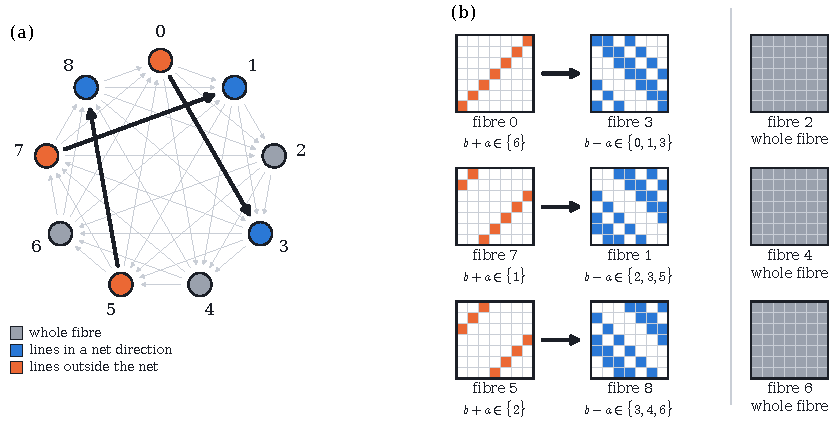
\includegraphics[width=\textwidth]{member.pdf}
\caption{A line-piece member of $\OM$ of degree $231$ (a solution of $Sx=-21x$); it is not centred.
(a)~The base $\Z_9$ with the tournament $i\to i+\{1,\dots,4\}$ (grey), points coloured by the kind of piece on their
fibre. The black arrows $0\to3$, $7\to1$, $5\to8$ are the decoupled pairs (Lemma~\ref{lem:decouple}).
(b)~The fibres, one row per pair, and the whole fibres $2$, $4$, $6$. In each $7\times7$ grid ($a$ indexes rows, $b$
columns) the coloured cells form $X$. Fibres $1$, $3$, $8$ meet $X$ in three lines $b-a=c$, a net direction; fibres
$0$, $5$, $7$ meet it in one line $b+a=c$, outside the net.}
\label{fig:member}
\end{figure}

\subsection{The census}
\begin{theorem}\label{thm:census}
The line-piece regular members of $\OM$ fall into $575$ isomorphism classes of degree $231$ and $603$ of degree
$210$, and the same holds for $\OP$. After complementing the members of degree $210$, this gives
$2\cdot(575+603)=2356$ strongly regular graphs with parameters $(442,231,120,121)$. They are pairwise
non-isomorphic, and $2256$ of them have trivial automorphism group.
\end{theorem}
\begin{proof}
By Lemma~\ref{lem:decouple}, a line-piece vector satisfies $Sx=\rho x$ if and only if (D1), (D2) and (D3) hold; the conditions are sufficient because, by (F1)--(F4), they
are all the components of $Sx=\rho x$. For $\rho=\pm21$, each arc and each set $T$ admits $14$ solutions of (D2).
Combining these with (D3) gives all line-piece members, and each resulting graph was also checked directly to be
strongly regular.

Isomorphism classes of members are $\Aut\Omega$-orbits~\cite[Lemma~2.4]{Plummer442}, so we keep one member per
orbit. Two independent canonical labellings confirm that the $2356$ graphs are pairwise non-isomorphic: a program
written for this purpose, and bliss~\cite{bliss} via igraph~\cite{igraph}. The second computation also gives the
automorphism groups in Table~\ref{tab:aut}. Expanding the representatives back to labelled vectors gives $5145$
vectors per degree and two-graph, as the frame decomposition predicts. As a control, the enumeration reproduces the
$15$ solutions per degree on $\OM$ of~\cite[Theorem~3.2]{Plummer442}, together with their graphs. The programs are
listed in Table~\ref{tab:programs}.
\end{proof}

\begin{table}[t]
\centering
{\small\setlength{\tabcolsep}{5pt}% generated by scripts/make_figures.py aut from data/census_props.tsv
\begin{tabular}{llrrrrr}
\toprule
 & & $|\Aut|=1$ & $|\Aut|=3$ & $|\Aut|=3$ & $|\Aut|=9$ & total \\
two-graph & degree & $1^{442}$ & $1^{10}\,3^{144}$ & $1^{1}\,3^{147}$ & $1^{1}\,3^{3}\,9^{48}$ & \\
\midrule
$\Omega_{\mathrm M}$ & $231$ & 570 & 5 (5) & -- & -- & 575 (5) \\
$\Omega_{\mathrm M}$ & $210$ & 558 & 3 (3) & 36 & 6 (6) & 603 (9) \\
$\Omega_{\mathrm P}$ & $231$ & 570 (1) & 5 (5) & -- & -- & 575 (6) \\
$\Omega_{\mathrm P}$ & $210$ & 558 & 3 (3) & 36 & 6 (6) & 603 (9) \\
\midrule
all & & 2256 (1) & 16 (16) & 72 & 12 (12) & 2356 (29) \\
\bottomrule
\end{tabular}
}
\bigskip
\caption{Automorphism groups of the $2356$ census graphs, by two-graph and degree (members of degree $210$ through
their complements). Each column gives $|\Aut|$ and the orbit lengths on the $442$ vertices. Numbers in brackets count
graphs known before the census: for $\OM$ the $14$ graphs of~\cite{Plummer442}, for $\OP$ $15$ members found earlier
with the same line-piece program ($14$ centred, $1$ rigid). So $29$ of the $2356$ graphs were known before.}
\label{tab:aut}
\end{table}

No census graph has a $22$-clique: the clique number is $13$ for $2192$ graphs and $14$ for $164$, all of the latter
members of $\OM$ of degree $231$ (Table~\ref{tab:programs}). Since $22=1+231/11$ is the Delsarte bound, no census graph
is geometric; in particular none is the block graph of a Steiner system $S(2,11,221)$, whose existence remains open. Nor is any of them the halved graph of a distance-regular graph on $884$
vertices with Delsarte cliques of size $22$~\cite{BCN}.

% ---------------------------------------------------------------------------------------------------------------
% Section for the joint paper: Mathon's family and the sporadicity of the line-piece members.
% \input{sporadic/sporadic.tex}. Needs amsthm environments theorem, lemma, proposition, corollary, remark, conjecture,
% the macros \F, \srg, \Aut, \OM, graphicx, booktabs, and the figures sporadic_gaps.pdf, sporadic_reduction.pdf
% (scripts/sporadic_figs.py). Claims are checked by scripts/sporadic_check.py (slope lemma for q = 7, 23; pair equations
% on the 14 graphs of [Plummer442]); the search is plummer/m23 (mitm.py, glob.py), log in plummer/m23/results/SUMMARY.txt.
% Uses labels sec:template (the template (Definition def:template) and Mathon blocks (M1), (M2)) and sec:decoupling.
% Standard facts are cited, not reproved; what is new is proved here (see the note, Section "What is cited").

\section{Sporadicity of standard line pieces}\label{sec:sporadic}

Mathon's construction~\cite[Theorem~4.1]{Mathon1978} (see also~\cite{SeberryWhiteman1988}) works for every prime power
$q\equiv3\pmod4$ such that a conference graph on $p=q+2$ vertices exists. For every such base graph and every skew
Latin square of order $p$, it gives a regular two-graph on $pq^2+1$ points with Seidel eigenvalues $\pm q\sqrt p$. For
$q$ prime this two-graph is an instance of the template (Lemma~\ref{lem:mathon-instance}). In this section $\Omega_q$
denotes any of these two-graphs; all results hold for all of them, except Proposition~\ref{prop:q23h}. As in
Section~\ref{sec:template}, a regular member has $Sx=\rho x$ with $\rho=\pm q\sqrt p$, so $p$ is a square. We write
\[q=s^2-2,\qquad p=s^2,\qquad \rho=\eta qs\quad(\eta=\pm1).\]
For $s=3,5,7,9,13,15,19,21,27,\dots$ this gives $q=7,\allowbreak 23,\allowbreak 47,\allowbreak 79,\allowbreak
167,\allowbreak 223,\allowbreak 359,\allowbreak 439,\allowbreak 727,\dots$. For $s=15$ and $s=21$, $p$ is not a prime
power, so there is no Paley base; a conference graph on $225$ vertices exists~\cite{GoethalsSeidel1967}, and on $441$
vertices one can take the descendant $\srg(441,220,109,110)$ of $\OM$. The first case is $\Omega_7=\OM$, and the
second has $13226$ points (Table~\ref{tab:orders}).

Do the line-piece members of $\OM$ belong to a family that continues with $q$? For standard line pieces they do not,
and at $q=23$ no line pieces do; for arbitrary intercept sets and larger $q$ this rests on
Conjecture~\ref{conj:twoval}. Theorem~\ref{thm:sporadic} shows that standard line pieces (Section~\ref{ssec:lines}) give regular members only for
$s=3$, in every template two-graph (Remark~\ref{rem:alltemplates}). The reason is a coincidence between two pairs of
small integers (Figure~\ref{fig:gaps}). Proposition~\ref{prop:hinv} describes, for every $q$, the members fixed by the
scalar automorphism $h$, and reduces the search for them to a small exact problem. At $q=7$ the solutions of this
problem are exactly the $15+15$ centred members, that is, the graphs of~\cite{Plummer442}; at $q=23$ it has none
(Proposition~\ref{prop:q23h}).

\subsection{Slopes and partners}
We use the notation of Section~\ref{sec:template}: vertices $\infty$ and $(i,a,b)$, the Seidel matrix $S$ with $\infty$ isolated and blocks $S_{ij}$, and the Seidel matrix $\Sigma$ of the base.
A \emph{slope} is an element $m$ of $\F_q\cup\{\infty\}$, with the linear form $\ell_m$ of Section~\ref{sec:template}.
We split the slopes into
\[
\mathcal M=\{0\}\cup Q,\qquad \mathcal P=N\cup\{\infty\},
\]
and write $m^*=-m$ for $m\in\F_q^\times$, $0^*=\infty$, $\infty^*=0$, so that $m\mapsto m^*$ exchanges $\mathcal M$ and $\mathcal P$.
For $q=7$ the slopes in $\mathcal M$ are the net directions of $\OM$.
Recall $\chi'=\chi-\delta_0$, so $\chi'(0)=-1$, and let $\tilde\chi'(y)=\chi'(-y)$.
Convolution is $(\kappa*g)(y)=\sum_x\kappa(y-x)g(x)$.

The lines of the $q+1$ parallel classes of $\F_q^2$ give the orthogonal decomposition of the functions on a fibre into the constants and, for each slope $m$, the mean-zero functions of $\ell_m$:
\begin{equation}\label{eq:slopes}
f=\bar f+\sum_{m}g_m\circ\ell_m,\qquad \textstyle\sum_y g_m(y)=0.
\end{equation}
The sum of $f$ over the line $\ell_m=y$ is $q\bar f+q\,g_m(y)$.

\begin{lemma}[slope decomposition]\label{lem:slopes}
Let $g\colon\F_q\to\mathbb R$ be non-zero with mean zero.
\begin{enumerate}
\item $S_{ii}(g\circ\ell_m)=-q\,g\circ\ell_m$ for $m\in\mathcal M$ and $+q\,g\circ\ell_m$ for $m\in\mathcal P$.
\item Every row of $S_{ij}$, $i\ne j$, sums to $-q\Sigma_{ij}$, and every row of $S_{ii}$ sums to $0$.
\item For every fibre $j$ and slope $m$ there is exactly one fibre $i\ne j$ with $S_{ij}(g\circ\ell_m)\ne0$, and
\[
S_{ij}(g\circ\ell_m)=q\,\Sigma_{ij}\,(\kappa*g)\circ\ell_{m^*},\qquad \kappa=\begin{cases}\tilde\chi',& m^*\in\mathcal P,\\ \chi',& m^*\in\mathcal M.\end{cases}
\]
\end{enumerate}
We call $(j,m)$ and $(i,m^*)$ \emph{partners}.
Partnership is a perfect matching on the $p(q+1)$ pairs (fibre, slope), and every partner pair joins a slope in $\mathcal M$ to a slope in $\mathcal P$.
\end{lemma}

\begin{proof}
We use the blocks (M1) and (M2) of Section~\ref{sec:template}.
(i) Let $\psi$ be a non-trivial additive character of $\F_q$. On the function $\psi(\beta\ell_m)$, $\beta\ne0$, the block (M1) acts by a scalar, which the evaluation of the quadratic Gauss sum~\cite[Theorem~5.15]{LidlNiederreiter} gives as $-q\chi(m)$ for $m\in\F_q^\times$, $-q$ for $m=0$ and $q$ for $m=\infty$.
(ii) Each row of (M2) contains every value of $\chi'$ exactly $q$ times, and $\sum_y\chi'(y)=-1$.
(iii) Let $0<k<\tfrac{p-1}2$ and put $y=b'-ma'$.
If $m=c_k$, the sum over $a'$ gives $(S_{ij}(g\circ\ell_m))(a,b)=q\Sigma_{ij}(\tilde\chi'*g)(b+c_ka)$, a function of $\ell_{-c_k}$.
If $m\ne c_k$, then for fixed $y$ the argument of $\chi'$ runs over $\F_q$ as $a'$ does, and the result is $-\Sigma_{ij}\sum_yg(y)=0$.
The case $k=\tfrac{p-1}2$ is the same with $0\mapsto\infty$.
The transposed blocks map $-c_k\mapsto c_k$ and $\infty\mapsto0$, with convolution kernel $\chi'$.
Since $L$ is a skew Latin square, the labels $L(i,j)$, $j\ne i$, take each of the $q+1$ values $\pm1,\dots,\pm\tfrac{p-1}2$ once, and $\{c_k\}=Q$, $-Q=N$.
So the slopes of fibre $i$ are reached once each: $N$ from the positive labels, $Q$ from the negative ones, $\infty$ and $0$ from $\pm\tfrac{p-1}2$.
\end{proof}

For $q$ prime, Lemma~\ref{lem:slopes} is Lemma~\ref{lem:blocks}, written in
Mathon's coordinates: the line $D$ is $\ker\ell_m$, the space $F^D$ consists of the functions $g\circ\ell_m$ with
$\sum_yg(y)=0$, the partner of $(i,\ker\ell_m)$ is $(j,\ker\ell_{m^*})$, and $M_i=q\,\bar x_i$. In particular,
Lemma~\ref{lem:slopes}(iii) is (D1) for $\Omega_q$, and Lemma~\ref{lem:eigen} below is (D2)--(D3).

\begin{lemma}\label{lem:eigen}
Let $x\in\{\pm1\}^{q^2p+1}$ with $x_\infty=1$, and decompose each fibre $x_i$ as in~\eqref{eq:slopes} with means $\bar x_i$ and slope parts $g_{i,m}$.
Then $Sx=\rho x$ if and only if
\begin{enumerate}
\item[(M)] $\bar x=\rho^{-1}\one+v$ with $\Sigma v=-(\rho/q)\,v$, and
\item[(P)] for every partner pair $(i,m)$, $(j,m^*)$ with $m\in\mathcal M$,
\[
g_{j,m^*}=\frac{\Sigma_{ij}}{\eta s-1}\,\tilde\chi'*g_{i,m},\qquad\text{equivalently}\qquad g_{i,m}=\frac{\Sigma_{ij}}{\eta s+1}\,\chi'*g_{j,m^*}.
\]
\end{enumerate}
\end{lemma}

\begin{proof}
By Lemma~\ref{lem:slopes}, $S$ preserves the decomposition~\eqref{eq:slopes}.
The fibres form an equitable partition, so on fibre means $S$ acts by its quotient matrix $-q\Sigma$~\cite[\S9.3]{GodsilRoyle}, and the column of $\infty$ adds $x_\infty=1$.
This gives $\rho\bar x=-q\Sigma\bar x+\mathbf1$, which is (M) because $\Sigma\one=0$.
Since $v$ is an eigenvector of the symmetric matrix $\Sigma$ for $-\rho/q\ne0$ and $\Sigma\one=0$, we have $\one^\top v=0$, so the row of $\infty$ reads $q^2\sum_i\bar x_i=q^2p/\rho=\rho$, which holds because $\rho^2=q^2p$.
On a partner pair, the slope parts satisfy $(\rho+q)g_{i,m}=q\Sigma_{ij}\chi'*g_{j,m^*}$ and $(\rho-q)g_{j,m^*}=q\Sigma_{ij}\tilde\chi'*g_{i,m}$.
These two equations are equivalent, because $\chi'*\tilde\chi'=(q+1)\delta_0-1$ acts as $q+1$ on mean-zero functions and $(\rho+q)(\rho-q)=q^2(q+1)$.
\end{proof}

\subsection{Line pieces}\label{ssec:lines}
A \emph{standard line piece} in a fibre is a set $\ell_m^{-1}(T)$ with $T$ a translate of a union of some of $\{0\}$, $Q$, $N$; a general line piece (Section~\ref{sec:decoupling}) allows any $T$.
The centred pieces of~\cite{Plummer442} are those with $T$ itself such a union, and the census members of Section~\ref{sec:census} use translates.
We say $T$ is \emph{two-valued} if $\chi'*\one_T$ takes exactly two values; their difference is the \emph{gap}.

\begin{remark}[why $q=7$]\label{rem:q7}
The simplest pieces already show the mechanism. If on a matched arc the head fibre meets $X$ in a single line,
$g_b=1-2\delta_c$, then (D2) makes $\tilde g_a$ two-valued with gap $4q/|q-\rho|$. So $g_a$ is $\pm1$-valued only if
$\rho=3q$. Likewise, a single line in the tail fibre forces $\rho=-3q$. Since $\rho=\pm q\sqrt p$, either case gives
$p=9$, $q=7$. The coincidence is visible in the graph $\mathrm A_1$ of~\cite[Table~1]{Plummer442}: fibre $1$ is
$\ell_1^{-1}(Q)$, and its partner, fibre $7$, is $\ell_6^{-1}(\{0\})$. The sets $-Q=N$ and $\{0\}$ have gaps $4=s+1$
and $2=s-1$, as (P) requires for $\rho=-21$. Theorem~\ref{thm:sporadic} is the general form of this observation.
\end{remark}

\begin{theorem}\label{thm:sporadic}
Let $q=s^2-2$ be as above, and let $X$ be a set of vertices of $\Omega_q$, not containing $\infty$, that meets every fibre in the empty set, the whole fibre or a standard line piece.
If switching with respect to $X$ gives a regular graph, then $q=7$.
\end{theorem}

\begin{proof}
Let $x$ be the switching vector, so $Sx=\rho x$ with $\rho=\eta qs$.
By (M), and as $\one^\top v=0$ (proof of Lemma~\ref{lem:eigen}), $\sum_i\bar x_i=p/\rho=\eta s/q$.
This is not an integer, because $\gcd(s,q)=\gcd(s,2)=1$ and $q>1$.
So some fibre $i$ is not constant, and $x_i=1-2\cdot\one_T\circ\ell_m$ for a slope $m$ and a set $T\ne\emptyset,\F_q$.
Then $g_{i,m}=-2(\one_T-|T|/q)\ne0$.
Let $(j,m^*)$ be the partner of $(i,m)$.
Both convolution kernels in (P) are invertible on mean-zero functions, so $g_{j,m^*}\ne0$.
Fibre $j$ is therefore not constant, its slope is $m^*$, and $g_{j,m^*}=-2(\one_U-|U|/q)$ for some set $U$.
Now (P) says that $\kappa*\one_T$, with $\kappa=\chi'$ or $\tilde\chi'$, is a constant plus a multiple of
$\one_U$, the multiple being $\pm(s-1)$ or $\pm(s+1)$. So $T$ (if $\kappa=\chi'$) or $-T$ (if $\kappa=\tilde\chi'$)
is two-valued with gap $s-1$ or $s+1$. Translation does not change the values, and $-Q=N$. Using
$\chi*\chi=1-q\delta_0$, the values of $\chi'*\one_T$ for the six proper non-empty unions of $\{0\},Q,N$ are:
\[
\begin{array}{l|cccccc}
T&\{0\}&Q&N&\{0\}\cup Q&\{0\}\cup N&Q\cup N\\\hline
\text{at }0&-1&-\tfrac{q-1}2&\tfrac{q-1}2&-\tfrac{q+1}2&\tfrac{q-3}2&0\\
\text{on }Q&1&-1&-1&0&0&-2\\
\text{on }N&-1&1&-1&0&-2&0\\\hline
\text{gap}&2&\text{(3 values)}&\tfrac{q+1}2&\tfrac{q+1}2&\text{(3 values)}&2
\end{array}
\]
So the possible gaps are $2$ and $\tfrac{q+1}2=\tfrac{(s-1)(s+1)}2$.
Now $2\in\{s-1,s+1\}$ forces $s=3$ or $s=1$, and $\tfrac{(s-1)(s+1)}2=s\pm1$ forces $s\mp1=2$, that is, again $s=3$ or $s=1$. The case $s=1$ gives $q=-1$, so $s=3$.

The argument after the first paragraph uses only that fibre $i$ is a standard line piece and that its partner $j$ is a
line piece; by the second form of (P) the roles of $i$ and $j$ can be exchanged. So for $s\ne3$ no line-piece regular
member of $\Omega_q$ has a fibre that is a standard line piece, and Conjecture~\ref{conj:twoval} is needed only for
members whose non-constant fibres are all non-standard.
\end{proof}

\begin{remark}[all template two-graphs]\label{rem:alltemplates}
For any template data with $q$ prime, call a line piece $g_i\circ\theta_i$ \emph{standard} if $\{y:g_i(y)=-1\}$ is a
translate of a union of some of $\{0\},Q,N$. This does not depend on the choice of $\theta_i$: replacing $\theta_i$ by
$\lambda\theta_i$ multiplies the set by $\lambda$, and $\lambda Q\in\{Q,N\}$. The class is also preserved by the
affine changes of variable below. The proof of Theorem~\ref{thm:sporadic} uses only the row of $\infty$ and the pair
equations (P). Both have analogues for any template data with $q$ prime and $p=s^2$. (D3) gives $q\sum_iM_i=\rho$, hence the same non-integrality, and
(D1) gives the partner fibre. For (P): since $\one_N=\tfrac12(\one+\tilde\chi')$ and $\one_{\{0\}\cup Q}=\tfrac12(\one-\tilde\chi')$ (as
$\chi(-1)=-1$), on mean-zero functions convolution with $\one_N$ is $\tfrac12$ times convolution with $\tilde\chi'$, and
convolution with $\one_{\{0\}\cup Q}$ is $-\tfrac12$ times it. After the affine change of variable that takes $N$ or
$\{0\}\cup Q$ to $T_{ab}$, equation (D2) therefore becomes (P) with $\Sigma_{ij}$ replaced by $-\varepsilon_{ab}$, the
Seidel entry of the base. Hence Theorem~\ref{thm:sporadic} holds for every template two-graph, in
particular for $\OP$ and the other $d=1$ two-graphs with $\Pal(q^2)$ fibres of~\cite[Section~6.5]{K833}.
\end{remark}

\begin{figure}[t]
\centering
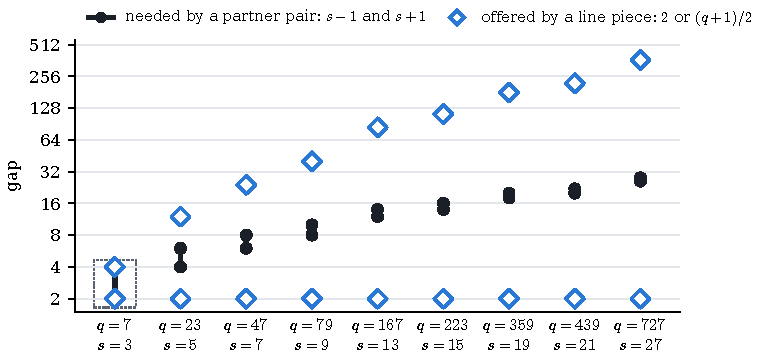
\includegraphics[width=0.78\textwidth]{sporadic_gaps.pdf}
\caption{Why standard line pieces work only for $q=7$.
In a line-piece regular member, each partner pair of fibres (Lemma~\ref{lem:slopes}) forces the intercept set $T$ of a line piece to be two-valued with gap $s-1$ or $s+1$ (black).
Standard line pieces offer only the gaps $2$ and $(q+1)/2$ (blue).
The two pairs agree only for $s=3$ (dashed box).
In every other member of Mathon's family, $s\pm1$ lies strictly between them.}
\label{fig:gaps}
\end{figure}

\begin{remark}\label{rem:twovalued}
The hypothesis on $T$ is used only to determine the possible gaps. For $q\in\{7,11,19,23,31\}$, an enumeration of all
$2^q$ subsets of $\F_q$ shows that the two-valued sets are exactly the translates of $\{0\}$, $N$, $\{0\}\cup Q$ and
$\F_q^\times$, with gaps $2$ and $\tfrac{q+1}2$; Conjecture~\ref{conj:twoval} asserts this for all $q$. Hence at
$q=23$ the conclusion of Theorem~\ref{thm:sporadic} holds for every $X$ that meets each fibre in a union of parallel
lines, whatever the intercepts. Proposition~\ref{prop:q23all} proves this independently for all template data.
\end{remark}

\subsection{Members fixed by \texorpdfstring{$h$}{h}}
Let $\omega$ generate $Q$, and let $h$ act by $(i,a,b)\mapsto(i,\omega a,\omega b)$ and fix $\infty$.
The blocks (M1) and (M2) are invariant under this scaling, so $h$ is an automorphism of $\Omega_q$ that fixes every fibre.
For $q=7$ it is the subgroup $C_3$ of $\Aut\OM$ that fixes every fibre, and the members it fixes are the centred ones.
Line pieces with $T$ a union of $\{0\},Q,N$ are $h$-invariant, but an $h$-invariant member need not be made of line pieces.

An $h$-invariant vector is constant on the $h$-orbits of a fibre (the origin and the half-lines through it), so a few
numbers per fibre describe it, and $Sx=\rho x$ becomes linear conditions on these numbers that couple only partner
fibres. An $h$-invariant function on a fibre is determined by two kinds of values.
One is its value $e_0$ at the origin.
The others are, for each slope $m$ with direction $d_m=(1,m)$ or $d_\infty=(0,1)$, its values $f_m^\pm$ on the two half-lines $\{td_m:\chi(t)=\pm1\}$.
Put $\alpha_m=(f_m^++f_m^-)/2$ and $\delta_m=(f_m^+-f_m^-)/2$, so that exactly one of them is $\pm1$ and the other is $0$, and put $A=\sum_m\alpha_m$.
Let $\sigma$ be the $(q+1)\times(q+1)$ matrix with $\sigma_{mm}=0$ and $\sigma_{mm'}=\chi(\ell_m(d_{m'}))$ for $m\ne m'$.
It satisfies $\sigma\sigma^\top=qI$ (a conference matrix in the general sense; it is neither symmetric nor skew), by the same character-sum identity $\chi*\chi=1-q\delta_0$ as Paley's matrices~\cite{Paley1933}.
Put $P=\sigma\delta$, i.e.\ $P_m=\sum_{m'\ne m}\sigma_{mm'}\delta_{m'}$.

\begin{proposition}\label{prop:hinv}
Let $x$ be the switching vector of an $h$-invariant member of $\Omega_q$, with $Sx=\eta qs\,x$ and $x_\infty=1$.
\begin{enumerate}
\item On fibre $i$ the sums of $x_i$ over the lines of slope $m$ depend only on whether the intercept is $0$, in $Q$ or in $N$:
\[
\Lambda_{i,m}(0)=e_0+(q-1)\alpha_m,\qquad \Lambda_{i,m}(Q)=A-\alpha_m+P_m,\qquad \Lambda_{i,m}(N)=A-\alpha_m-P_m,
\]
with $e_0,\alpha,P,A$ those of fibre $i$.
\item Put $u=\Lambda(0)-\Lambda(Q)$, $v=\Lambda(0)-\Lambda(N)$ and $w=\Lambda(Q)-\Lambda(N)=2P$. For every partner
pair $(i,m)$, $(j,m^*)$ with $m\in\mathcal M$,
\[
u_{j,m^*}=\Sigma_{ij}\,\frac{\eta s+1}2\,w_{i,m},\qquad v_{i,m}=-\Sigma_{ij}\,\frac{\eta s-1}2\,w_{j,m^*}.
\]
\item Consequently every fibre satisfies, for each slope $m$, the local conditions
\[
\begin{cases}
v_m\equiv0\pmod{s-\eta}\ \text{and}\ |P_m|\le 2q/(s+\eta), & m\in\mathcal M,\\
u_m\equiv0\pmod{s+\eta}\ \text{and}\ |P_m|\le 2q/(s-\eta), & m\in\mathcal P.
\end{cases}
\]
They involve only $q$, $s$ and $\eta$, not $i$ or $\Sigma$.
\end{enumerate}
\end{proposition}

\begin{proof}
(i) The line $\ell_m=0$ consists of the origin and the two half-lines of slope $m$.
A line $\ell_m=y$ with $y\ne0$ meets the line through the origin of slope $m'\ne m$ in the single point $td_{m'}$, where $t=y/\ell_m(d_{m'})$.
That point lies on the half-line of sign $\chi(y)\sigma_{mm'}$.
Summing $\alpha_{m'}+\chi(y)\sigma_{mm'}\delta_{m'}$ over $m'\ne m$ gives the formula.
(ii) By the remark after~\eqref{eq:slopes}, $q\,g_{i,m}=\Lambda_{i,m}-q\bar x_i$.
Write this mean-zero function as $a(\delta_0-1/q)+b\chi$.
Then $u=a-b$, $v=a+b$ and $w=2b$.
In the basis $(\delta_0-1/q,\chi)$, convolution with $\chi'$ acts by $(a,b)\mapsto(-a-qb,\ a-b)$, and convolution with $\tilde\chi'$ by $(a,b)\mapsto(-a+qb,\ -a-b)$; both follow from $\chi*\chi=1-q\delta_0$.
Comparing the $\chi$-coefficients in the two forms of (P) gives (ii).
(iii) By (ii), $u_{j,m^*}=\pm(s+\eta)P_{i,m}$ and $v_{i,m}=\pm(s-\eta)P_{j,m^*}$.
Moreover $|u|,|v|\le2q$, since every line sum lies in $[-q,q]$.
\end{proof}

At $q=7$ the line pieces of~\cite{Plummer442} satisfy (ii) with one side zero.
For example, fibres $1$ and $7$ of $\mathrm A_1$ (Remark~\ref{rem:q7}) have $(u,v,w)=(14,0,-14)$ and $(-14,-14,0)$, and $\Sigma_{17}=-1$ (Figure~\ref{fig:reduction}(a)).
A general $h$-invariant fibre mixes the states $\alpha$ and $\delta$ on different slopes, and (ii) couples it to $q+1$ other fibres.

\paragraph{The two-graph $\Omega_{23}$.} For $q=23$ we take the base $\Pal(25)$ and label $\F_{25}=\F_5[i]$, $i^2=2$,
by $\Z_{25}$ via $yi+z\mapsto5y+z$. The skew Latin square is the circulant one, $L(a,b)=b-a$ reduced to
$\pm1,\dots,\pm12$. Translating the labels by $5$ is the field translation by $i$. This is an automorphism of
$\Pal(25)$ that preserves $L$, and (M1), (M2) depend on the fibres only through $\Sigma$ and $L$, so it induces an
automorphism $t$ of $\Omega_{23}$ of order $5$.

\begin{proposition}\label{prop:q23h}
$\Omega_{23}$ has no regular member fixed by $h$: there is no $h$-invariant member that is an
$\srg(13226,6670,3363,3364)$ or an $\srg(13226,6555,3248,3249)$.
\end{proposition}
\begin{proof}
An $h$-invariant fibre is determined by its value at the origin and its values on the two half-lines of each slope,
which gives $2\cdot4^{q+1}$ states. By Proposition~\ref{prop:hinv}, we must choose one state per fibre so that (ii)
and (M) hold. Neither step below assumes that fibres are line pieces.

First, by meet-in-the-middle over the slopes, we list the \emph{local patterns}: the states that satisfy the local
conditions (iii), which are the same for every fibre. Second, we choose one local pattern per fibre by depth-first
search with forward checking. The constraints are the two equations of (ii) on each of the $p(q+1)/2$ partner pairs;
condition (M) is checked on complete assignments, and the symmetry $t$ is broken. Every solution is rebuilt as a vector
$x\in\{\pm1\}^{q^2p+1}$, and $Sx=\rho x$ is checked directly. Table~\ref{tab:search} gives the sizes. For $q=23$ there
is no solution for either sign of $\rho$.
\end{proof}

\begin{table}[h]
\centering\small
\begin{tabular}{rrrrrr}
\toprule
$q$ & $\rho$ & degree & local patterns & search nodes & solutions\\
\midrule
$7$ & $-21$ & $231$ & $6256$ & $418\,869$ & $15$\\
$7$ & $21$ & $210$ & $6256$ & $417\,337$ & $15$\\
$23$ & $-115$ & $6670$ & $206\,632$ & $284\,271\,840$ & $0$\\
$23$ & $115$ & $6555$ & $189\,142$ & $276\,655\,619$ & $0$\\
\bottomrule
\end{tabular}
\caption{The exact search for $h$-invariant members; at $q=23$ a fibre has $2\cdot4^{24}\approx5.6\cdot10^{14}$ states.}
\label{tab:search}
\end{table}

\begin{remark}[controls]\label{rem:search}
At $q=7$ the same search returns exactly the $15+15$ centred members, that is, the switching sets of the graphs
of~\cite{Plummer442} and their images under $\Aut\OM$. Requiring invariance under all of $\langle h,t\rangle$, with
$t\colon(i,u)\mapsto(i+3,u)$ of order $3$ (Section~\ref{sec:census}), leaves
exactly the graphs $\mathrm B_4,\dots,\mathrm B_9$ of~\cite[Table~1]{Plummer442}. At $q=23$ the two searches under
$\langle h\rangle$ took $47$ and $45$ CPU hours. Under $\langle h,t\rangle$, with $t$ the automorphism of order $5$ above, the search is much shorter: degree $6555$ is
excluded by (M) and the integrality of the fibre sums alone, and degree $6670$ after $63$ search nodes.
\end{remark}

\begin{figure}[t]
\centering
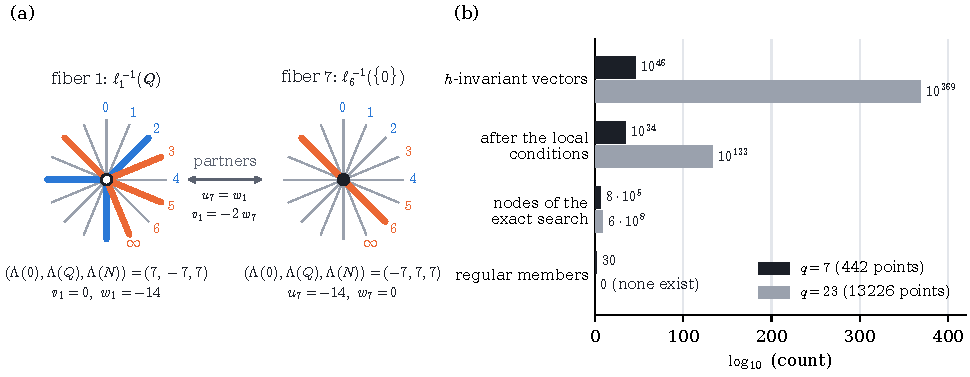
\includegraphics[width=\textwidth]{sporadic_reduction.pdf}
\caption{The local structure of $h$-invariant members, and the search it makes possible.
(a)~Two fibres of the graph $\mathrm A_1$ of~\cite{Plummer442} that are partners (Lemma~\ref{lem:slopes}), drawn by their $h$-orbits.
The dot is the origin, filled if it is switched.
Each diameter is the line through the origin of one slope, blue for $\mathcal M=\{0\}\cup Q$ and orange for $\mathcal P=N\cup\{\infty\}$.
Its half towards the label is $\{td_m:t\in Q\}$, and a half is drawn thick when it is switched.
Fibre $1$ is the line piece $\ell_1^{-1}(Q)$, which has the state $\delta$ on every slope except $1$.
Below each fibre are its line sums on the partner slopes $1$ and $6$, which satisfy the pair equations of Proposition~\ref{prop:hinv}(ii).
(b)~Sizes on a logarithmic scale for $q=7$ and $q=23$, both degrees together: all $h$-invariant switching vectors,
$(2\cdot4^{q+1})^p$ (out of $2^{441}$ and $2^{13225}$ in all); those whose fibres are all local patterns; search nodes
(for $q=23$ after breaking a symmetry of order $5$); and regular members found ($30$ centred members at $q=7$, none at
$q=23$).}
\label{fig:reduction}
\end{figure}


\subsection{Every instance at \texorpdfstring{$q=23$}{q=23}}\label{ssec:q23all}
Proposition~\ref{prop:q23h} concerns one two-graph. Lemma~\ref{lem:decouple} holds for every instance of the template,
which gives a statement on line pieces for all of them, with arbitrary intercept sets.

\begin{proposition}\label{prop:q23all}
Let $\Omega$ be the two-graph of any template data with $q=23$ ($n=13226$). There is no line-piece vector $x$ with
$Sx=\pm115\,x$. Hence $\Omega$ has no $\srg(13226,6555,3248,3249)$ and no $\srg(13226,6670,3363,3364)$ member whose
switching set meets every fibre in a union of parallel lines.
\end{proposition}
\begin{proof}
By (D1), every non-constant fibre lies on a matched arc and satisfies (D2). If $T'=\alpha T+\beta$, then $(g_a,g_b)$
solves (D2) for $T$ if and only if $(g_a',g_b')$ with $g_a'(y)=g_a(\alpha^{-1}(y-\beta))$ and
$g_b'(y)=g_b(\alpha^{-1}y)$ solves it for $T'$. So it suffices to take $T\in\{Q,N,\{0\}\cup Q,\{0\}\cup N\}$. An
exhaustive search over all $2^{23}$ functions $g$, for these four sets and both $\rho=\pm115$, finds no solution. Hence
every fibre is constant, $M_i=23c_i$ with $c_i=\pm1$, and (D3) reads
$1+23\sum_{j\ne i}\varepsilon_{ij}c_j=\pm5\cdot23\,c_i$, which is impossible modulo $23$.
\end{proof}
As a control, the same program at $q=7$ finds $14$ solutions per arc and $5145$ vectors per degree, as in the census.
Independently, CP-SAT~\cite{CPSAT} finds no regular member of $\Omega_{23}$ (Section~\ref{sec:sporadic}) in the line-piece
model of~\cite{Plummer442}, where every fibre is empty, whole, or $\ell_m^{-1}(T)$ with $T$ a union of $\{0\},Q,N$, for
either degree.

% ---------------------------------------------------------------------------------------------------------------
\section{Verification, data and code}\label{sec:verification}
Table~\ref{tab:programs} lists, for each computational statement, the programs that check it: A.K.'s are in
\code{koval/}, D.P.'s in \code{plummer/}. Where both are named, the two programs were written independently.

\begin{table}[!ht]
\centering\small
\begin{tabular}{p{0.42\textwidth}p{0.5\textwidth}}
\toprule
statement & programs\\
\midrule
template two-graphs $\OM$, $\OP$; $S^2=pq^2I$ & A.K.: \code{P2\_family442.py}, \code{check\_template\_data.py}; $q=23$: \code{c5\_build23.py}\\
Mathon's blocks are template instances (Lemma~\ref{lem:mathon-instance}) & A.K.: \code{mathon\_literal\_blocks.py}
($q=3,7,23$, with a negative control); Mathon's printed matrices at $q=3$: \code{c1\_controls.py}\\
$\Aut\OP\cong C_3\times C_3$ & A.K.: \code{P3\_members.py} (nauty~\cite{nauty} on the descendant at $\infty$, the unique fixed point)\\
census, Theorem~\ref{thm:census} & A.K.: \code{P3\_members.py}, \code{gcanon.c}, \code{members.py}; D.P.:
\code{census\_props.py} (bliss), \code{frames.py} ($5145=15\cdot7^3$)\\
the $23$ two-graphs are pairwise non-isomorphic & A.K.: \code{f5.c} with \code{f5\_invariant.py}, \code{descinv.c} with \code{twograph23\_second.py}\\
no $22$-cliques (clique numbers $13$, $14$) & A.K.: \code{dcliq.c}, \code{make\_controls.py} (Steiner-block-graph controls), \code{cliques\_per\_graph.tsv};
D.P.: check of the $14$ graphs of~\cite{Plummer442}\\
slope lemma, pair equations (Section~\ref{sec:sporadic}) & D.P.: \code{sporadic\_check.py} ($q=7,23$; $504$ pairs on $14$
graphs), \code{sporadic\_figs.py}\\
$h$-invariant search (Proposition~\ref{prop:q23h}, Remark~\ref{rem:search}) & D.P.: \code{plummer/m23} (\code{mitm.py},
\code{glob.py}, \code{verify\_hit.py}; control at $q=7$ also \code{reduced.py})\\
Proposition~\ref{prop:q23all} & A.K.: \code{c3\_arcs.py}, \code{c4\_global.py} (controls: their runs at $q=7$); D.P.:
CP-SAT on the line-piece model of~\cite{Plummer442}, \code{plummer/m23/pieces.py}\\
two-valued sets (Remark~\ref{rem:twovalued}, Conjecture~\ref{conj:twoval}) & D.P.: \code{plummer/m23/twoval.py}\\
hashes and counts of the census files, clique numbers, orbit arithmetic & A.K.: \code{check\_numbers.py}\\
Tables~\ref{tab:orders}, \ref{tab:arcs}, \ref{tab:aut}; (F1)--(F3) block by block on $\OM$, $\OP$ and four random template data; (D3) on $48$ members & D.P.: \code{check\_paper442.py}\\
\bottomrule
\end{tabular}
\caption{Programs behind the computational statements. The census is stored as four graph6 files (in
\code{koval/data/koval442\_linepiece\_2356.zip}), with SHA-256 \code{46fe141c\ldots} ($\OP$, $231$), \code{8f91dba6\ldots}
($\OP$, $210$, complemented), \code{ab384ab8\ldots} ($\OM$, $231$) and \code{7e1207a4\ldots} ($\OM$, $210$, complemented);
the full hashes are in \code{koval/README.md}. Programs and data:
\url{https://github.com/dylan-plummer/srg442-line-pieces}.}
\label{tab:programs}
\end{table}
\FloatBarrier

\section{Open questions}\label{sec:open}
\begin{question}
Does any template two-graph on $13226$ points, or any two-graph from Mathon's Theorem~4.2, have a regular member? By
Proposition~\ref{prop:q23all}, the switching set of such a member of a template two-graph is not a union of parallel
lines on some fibre.
\end{question}
\begin{question}
Is the template two-graph with $\Pal(529)$ fibres on $13226$ points also free of $h$-invariant regular members?
(Theorem~\ref{thm:sporadic} already holds for it, Remark~\ref{rem:alltemplates}.)
\end{question}
\begin{conjecture}\label{conj:twoval}
For every prime $q\equiv3\pmod4$, the subsets $T\subseteq\F_q$ for which $\chi'*\one_T$ is two-valued are exactly the
translates of $\{0\}$, $N$, $\{0\}\cup Q$ and $\F_q^\times$ (checked for $q\in\{7,11,19,23,31\}$, Remark~\ref{rem:twovalued}).
\end{conjecture}
\begin{question}
Can an exact search reach members of $\Omega_{23}$ with less symmetry than $\langle h\rangle$, or other bases and skew Latin
squares at $q=23$?
\end{question}

\subsection*{Use of AI systems}
This work was done with substantial assistance from AI systems; they are not authors, and the authors are responsible
for all content. On the first author's side, the search and verification programs, the figures, the integration of
the two authors' material and a first draft of the text were produced in collaboration with an AI assistant (Claude
Opus 5.5, Anthropic) under the first author's direction. Separate AI sessions then reviewed the draft as a referee, as
a literature and citation check, and as a readability check, and all results were checked as described in
Section~\ref{sec:verification}. On the second author's side, the template and its analysis, the programs for the
census, for the comparison of the two-graphs and for the $q=23$ statements, and the first version of the corresponding
text were produced by AI coding agents working under the second author's direction, mainly Claude (Anthropic; models
Claude Fable and Claude Opus); Codex (OpenAI; model Luna) and Junie (JetBrains; model Astra) were used as independent
checkers, and one of them recomputed the census from the definitions with its own programs. No result is accepted on
the word of such a system: every graph of the census is certified by exact integer arithmetic, confirmed by programs
written independently on both authors' sides.

\begin{thebibliography}{99}\small
\bibitem{BrouwerTable} A.~E.~Brouwer, \emph{Parameters of strongly regular graphs},
\url{https://aeb.win.tue.nl/graphs/srg/srgtab.html}, accessed 28 October 2026.
\bibitem{BH2012} A.~E.~Brouwer and W.~H.~Haemers, \emph{Spectra of Graphs}, Universitext, Springer, New York, 2012,
doi:10.1007/978-1-4614-1939-6.
\bibitem{BvM2022} A.~E.~Brouwer and H.~Van~Maldeghem, \emph{Strongly Regular Graphs}, Encyclopedia Math.\ Appl.\ \textbf{182},
Cambridge Univ.\ Press, 2022, doi:10.1017/9781009057226.
\bibitem{BCN} A.~E.~Brouwer, A.~M.~Cohen and A.~Neumaier, \emph{Distance-Regular Graphs}, Springer, Berlin, 1989,
doi:10.1007/978-3-642-74341-2.
\bibitem{CalderbankKantor1986} R.~Calderbank and W.~M.~Kantor, \emph{The geometry of two-weight codes}, Bull.\ London Math.\
Soc.\ \textbf{18} (1986), 97--122, doi:10.1112/blms/18.2.97.
\bibitem{CPSAT} L.~Perron and F.~Didier, \emph{CP-SAT}, OR-Tools v9.15, Google,
\url{https://developers.google.com/optimization/cp/cp_solver/}.
\bibitem{igraph} G.~Cs\'ardi and T.~Nepusz, \emph{The igraph software package for complex network research}, InterJournal
Complex Systems \textbf{1695} (2006).
\bibitem{GodsilRoyle} C.~Godsil and G.~Royle, \emph{Algebraic Graph Theory}, Grad.\ Texts in Math.\ \textbf{207}, Springer,
2001, doi:10.1007/978-1-4613-0163-9.
\bibitem{GoethalsSeidel1967} J.~M.~Goethals and J.~J.~Seidel, \emph{Orthogonal matrices with zero diagonal}, Canad.\ J.\
Math.\ \textbf{19} (1967), 1001--1010, doi:10.4153/CJM-1967-091-8.
\bibitem{bliss} T.~Junttila and P.~Kaski, \emph{Engineering an efficient canonical labeling tool for large and sparse
graphs}, Proc.\ ALENEX 2007, SIAM, 2007, 135--149, doi:10.1137/1.9781611972870.13.
\bibitem{K833} A.~Kova\v{l}, \emph{A strongly regular graph with parameters $(833,416,207,208)$}, preprint, version~1.2,
Zenodo, 2026, doi:10.5281/zenodo.23811118.
\bibitem{LidlNiederreiter} R.~Lidl and H.~Niederreiter, \emph{Finite Fields}, 2nd ed., Encyclopedia Math.\ Appl.\ \textbf{20}, Cambridge Univ.\ Press, 1997.
\bibitem{Mathon1978} R.~Mathon, \emph{Symmetric conference matrices of order $pq^2+1$}, Canad.\ J.\ Math.\ \textbf{30}
(1978), 321--331, doi:10.4153/CJM-1978-029-1.
\bibitem{nauty} B.~D.~McKay and A.~Piperno, \emph{Practical graph isomorphism, II}, J.\ Symbolic Comput.\ \textbf{60}
(2014), 94--112, doi:10.1016/j.jsc.2013.09.003.
\bibitem{NelsonSwartz2025} S.~R.~Nelson and E.~Swartz, \emph{Character theoretic techniques for nonabelian partial
difference sets}, arXiv:2507.23039, version~3, June 2026.
\bibitem{Paley1933} R.~E.~A.~C.~Paley, \emph{On orthogonal matrices}, J.\ Math.\ Phys.\ \textbf{12} (1933), 311--320, doi:10.1002/sapm1933121311.
\bibitem{Plummer442} D.~Plummer, \emph{Strongly regular graphs with parameters $(442,231,120,121)$ from Mathon's
conference two-graph}, preprint, 2026, \url{https://github.com/dylan-plummer/srg442}, commit \code{ab9b114}.
\bibitem{SeberryWhiteman1988} J.~Seberry and A.~L.~Whiteman, \emph{New Hadamard matrices and conference matrices obtained
via Mathon's construction}, Graphs Combin.\ \textbf{4} (1988), 355--377, doi:10.1007/BF01864173.
\bibitem{Seidel1976} J.~J.~Seidel, \emph{A survey of two-graphs}, Colloq.\ Int.\ Teorie Combinatorie (Roma, 1973), Tomo I,
Atti dei Convegni Lincei \textbf{17}, Accad.\ Naz.\ Lincei, 1976, 481--511.
\bibitem{Taylor1977} D.~E.~Taylor, \emph{Regular $2$-graphs}, Proc.\ London Math.\ Soc.\ (3) \textbf{35} (1977), 257--274,
doi:10.1112/plms/s3-35.2.257.
\end{thebibliography}
\end{document}
